%%%%%%%%%%%%%%%%%%%%%%%%%%%%%%%%%%%%%%%%%%%%%%%%%%%%%%%%%%
%%
%% MARK: Title & Data
%%
%%%%%%%%%%%%%%%%%%%%%%%%%%%%%%%%%%%%%%%%%%%%%%%%%%%%%%%%%%

\chapter*{\S B20. The Geodesics of the $2$-Torus}
\setcounter{footnote}{0}

%%%%%%%%%%%%%%%%%%%%%%%%%%%%%%%%%%%%%%%%%%%%%%%%%%%%%%%%%%
%%
%% MARK: Abstract
%%
%%%%%%%%%%%%%%%%%%%%%%%%%%%%%%%%%%%%%%%%%%%%%%%%%%%%%%%%%%

\begin{abstract}
  We describe the space of geodesic trajectories of the $2$-torus,
  and we exhibit its natural parasymplectic structure.
\end{abstract}

%%%%%%%%%%%%%%%%%%%%%%%%%%%%%%%%%%%%%%%%%%%%%%%%%%%%%%%%%%
%%
%% MARK: The Space Of Geodesics Of The 2-Torus
%%
%%%%%%%%%%%%%%%%%%%%%%%%%%%%%%%%%%%%%%%%%%%%%%%%%%%%%%%%%%

It is well known that,
if the space of (oriented) \emph{geodesic trajectories} (\emph{a.k.a.} unparametrized geodesics) of a manifold is a manifold,
then this manifold is naturally symplectic.
A famous example is the geodesics of the sphere $\Sph^2$,
for which the space of geodesics is also $\Sph^2$, equipped with the standard surface element%
\footnote{For a judicious choice of constant.}
The mapping from the unit bundle $\UnitBundle{\Sph^2} = \{(x,u)\in \Sph^2 \times \Sph^2 \mid u \cdot x = 0\}$ to $\Geod(\Sph^2)$ is realized by the moment map $\ell : (x,u) \mapsto x \wedge u$.

Now,

\uline{Question} What about the space of geodesics of the torus $\Torus^2$?

It is certainly not a manifold because of the mixture of closed and non-closed geodesics.
And what about the canonical symplectic structure?
Does something of it remain?
And what?

In the following,
we denote by $\Proj : \RR^2 \to \Torus^2 = \RR^2/\ZZ^2$ the projection.

As usual in symplectic geometry,
we realize the space $\Geod(\Torus^2)$ as the space of characteristics of the presymplectic form $d\lambda$ on the unit bundle $\U\Torus^2 \simeq \Torus^2 \times \Sph^1$,
where
$$
  \lambda (\delta y) = u \cdot \delta x,
  $$
with $y = (\Proj(x),u) \in \U\Torus^2$ and $\delta y = (\Der(\Proj)_x(\delta x), \delta u) \in T_y\U\Torus^2$.
Thus,
the characteristics of $d\lambda$ are the submanifolds
$$
  \gamma = \big( \Proj \{x+tu\}_{t\in \RR}, u \big),
  $$
when $(\Proj(x),u)$ is a point in $\U\Torus^2$.
We denote by $\pi$ the projection from $\U\Torus^2$ to $\Geod(\Torus^2)$,
$$
  \pi : (\Proj(x),u) \mapsto \big( \Proj \{x+tu\}_{t\in \RR}, u \big).
  $$

The space $\Geod(\Torus^2)$ of unparametrized geodesics of the $2$-torus is naturally a bundle%
\footnote{But not a fiber bundle.}
over the circle $\Sph^1$,
thanks to the projection
$$
  \Proj_2 : \big( \Proj \{x+tu\}_{t\in \RR}, u \big) \mapsto u.
  $$
The preimage $\Geod_u(\Torus^2) = \Proj_2^{-1}(u)$ is the space of all geodesics with slope $u$,
that is,
the torus $T_u = \Torus^2/\Delta_u$,
where $\Delta_u = \Proj(\RR u)$.
Precisely,
$T_u$ is a \emph{rational torus} (a circle) if $u$ is a rational vector,
that is,
if $\RR u \cap \ZZ^2 \simeq \ZZ$.
And $T_u$ is an \emph{irrational torus} \cite{DI83} if $\RR u \cap \ZZ^2 = \{0\}$.

$$
  \begin{tikzcd}[column sep=1.5em, row sep=3em, every label/.append style = {font = \small}]
  \U\RR^2 \arrow[rr, "\pi"]  \arrow[d, swap, "\ "]       &                         & \Geod(\RR^2) \arrow[d,"\ "]   \\
  \U\Torus^2 \arrow[rr, "\pi"] \arrow[dr,swap,"\Proj_2"]   &                         & \Geod(\Torus^2) \arrow{dl}{\Proj_2} \\
  &          \Sph^1            &
  \end{tikzcd}
  $$

\begin{Article}{Parasymplectic structure on $\Geod(\Torus^2)$.}{}
  There exists a closed $2$-form $\omega$ on $\Geod(\Torus^2)$ such that $\pi^*(\omega) = d\lambda$.
  We say that $\omega$ is parasymplectic.%
  \footnote{The analysis of $\Diff(\Geod(\Torus^2),\omega)$ and the universal moment map \cite[\textsection\,9.14]{PIZ13} is discussed in ``Diffeomorphisms of $\Geod(\Torus^2)$'',
  in these notes.}
\end{Article}

\Note It is noteworthy that,
in spite of the singularities of the space of geodesics,
some closed and diffeomorphic to the circle (indexed by $\QQ$) and others unclosed and diffeomorphic to $\RR$,
the presymplectic form $d\lambda$ descends to a smooth closed $2$-form on the quotient $\Geod(\Torus^2)$.
And that is the main fact to which we wish to draw your attention.

\begin{proof}
  We use the criterion in \textsection\,6.38 of \cite{PIZ13} on $d\lambda$.
  Let $P: r \mapsto (z_r,u_r)$ and $P' : r \mapsto (z'_r,u'_r)$ be two plots of $\U\Torus^2$,
  defined on the same domain and such that $\pi \circ P = \pi \circ P'$.
  That is,
  $$
    \big( \Proj \{x_r+tu_r\}_{t\in \RR}, u_r \big) = \big( \Proj \{x'_r+tu'_r\}_{t\in \RR}, u'_r \big).
    $$
  Thus,
  $u'_r = u_r$ and $\Proj \{x'_r+tu_r\}_{t\in \RR} = \Proj \{x_r+tu_r\}_{t\in \RR}$.
  Then, $x'_r = x_r + f(r) u_r$,
  with $f(r) = u_r \cdot (x'_r - x_r)$,
  and $f$ is smooth.
  Next,
  \begin{align*}
    \lambda(P')_r(\delta r) & =  u_r \cdot \big(\delta x_r + df_r(\delta r) u_r + f(r) \delta u_r\big) \\
    & =  \lambda(P)_r(\delta r) + df_r(\delta r).
  \end{align*}
  That is,
  $\lambda(P') = \lambda(P) + df$.
  Therefore,
  $d(\lambda(P')) = d(\lambda(P))$.
  By applying \textsection\,6.38 of \cite{PIZ13},
  there exists $\omega \in \DForms^2(\Geod(\Torus^2))$ such that $\pi^*(\omega) = d\lambda$ and $d\omega = 0$.
\end{proof}

\vfill
\centerline{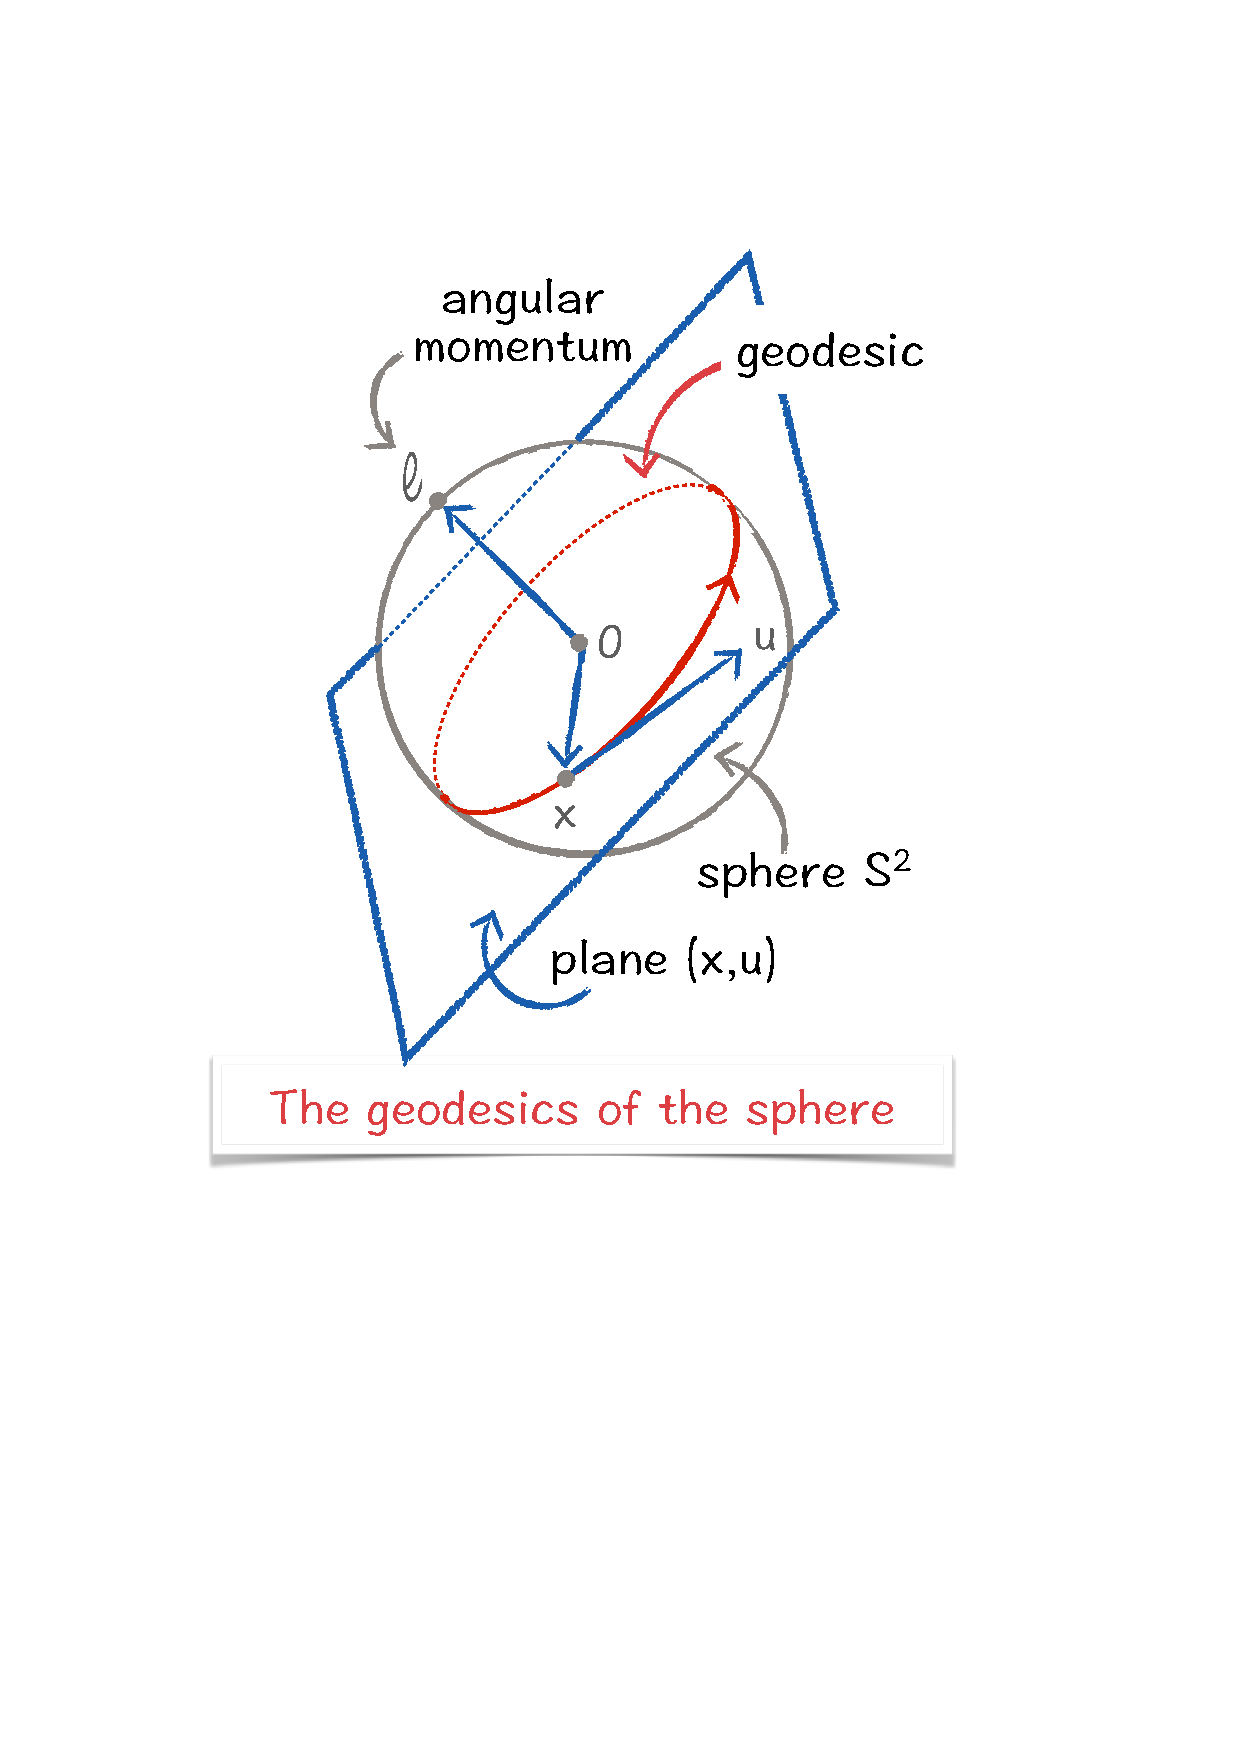
\includegraphics[width=.48\textwidth]{Figures/geodesic-sphere.pdf}}
\vfill
